% 2.1.Download.tex
%	Last update: 2019/07/22 F.Kanehori
%newpage
\subsection{GkrZwDollfzZLadk}
\label{subsec:Download}

\noindent
\KLUDGE まずSpringhead Library\KLUDGE をGitHub\KLUDGE からダウンロード(clone)\KLUDGE してください。
\KLUDGE 以下、ダウンロードするディレクトリを\SprTop{}\KLUDGE として説明を進めます。

\medskip
\ifLwarp
	\begin{figure}[h]
	    \begin{center}
	    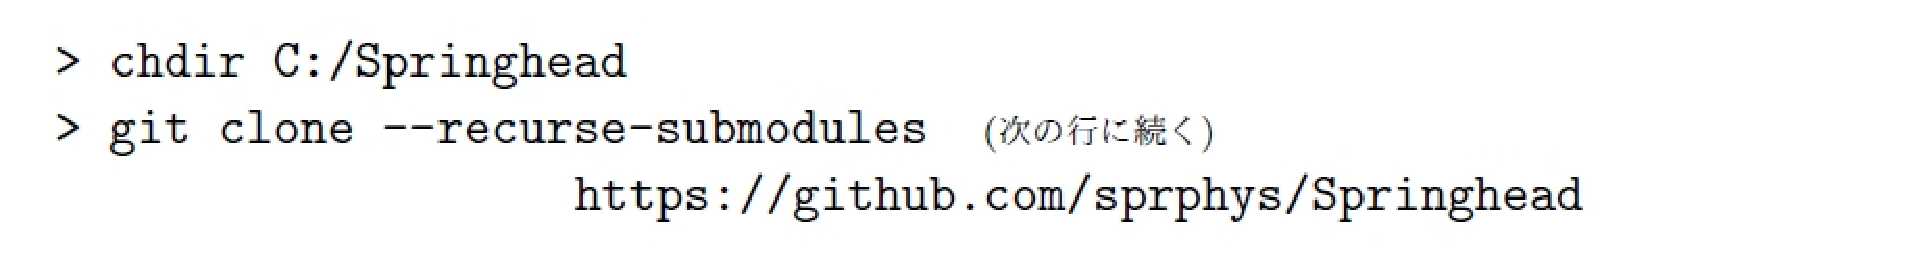
\includegraphics[width=\textwidth]{fig/command-2-1-a.eps}
	    \end{center}
	    \label{fig:DownloadTree}
	\end{figure}
\else
\begin{narrow}[15pt]
	\CmndBox{%
		\textgreater  chdir C:/Springhead\\
		\textgreater  git clone --recurse-submodules\Cont\\
		\Hskip{100pt}https://github.com/sprphys/Springhead
	}
\end{narrow}
\fi
\medskip
\KLUDGE サブモジュールを選択する場合は、
\ifLwarp
	\begin{figure}[h]
	    \begin{center}
	    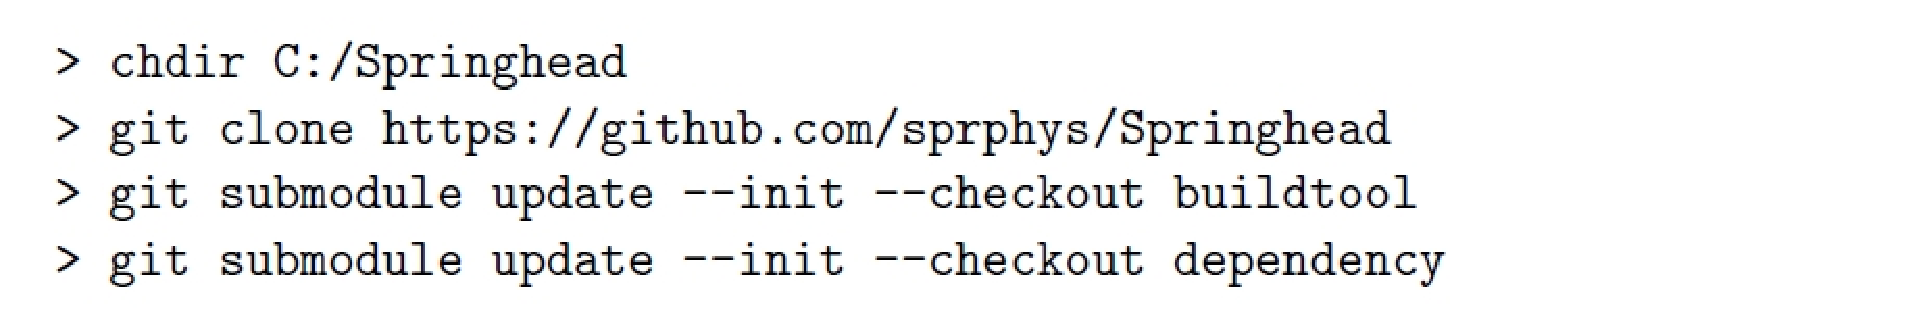
\includegraphics[width=\textwidth]{fig/command-2-1-b.eps}
	    \end{center}
	    \label{fig:DownloadTree}
	\end{figure}
\else
\begin{narrow}[15pt]
	\CmndBox{%
		\textgreater  chdir C:/Springhead\\
		\textgreater  git clone https://github.com/sprphys/Springhead\\
		\textgreater  git submodule update --init --checkout buildtool\\
		\textgreater  git submodule update --init --checkout dependency
	}
\end{narrow}
\fi
\medskip
GUI\KLUDGE の場合は、
\begin{narrow}[15pt]
	\begin{figure}[h]
	\begin{center}
	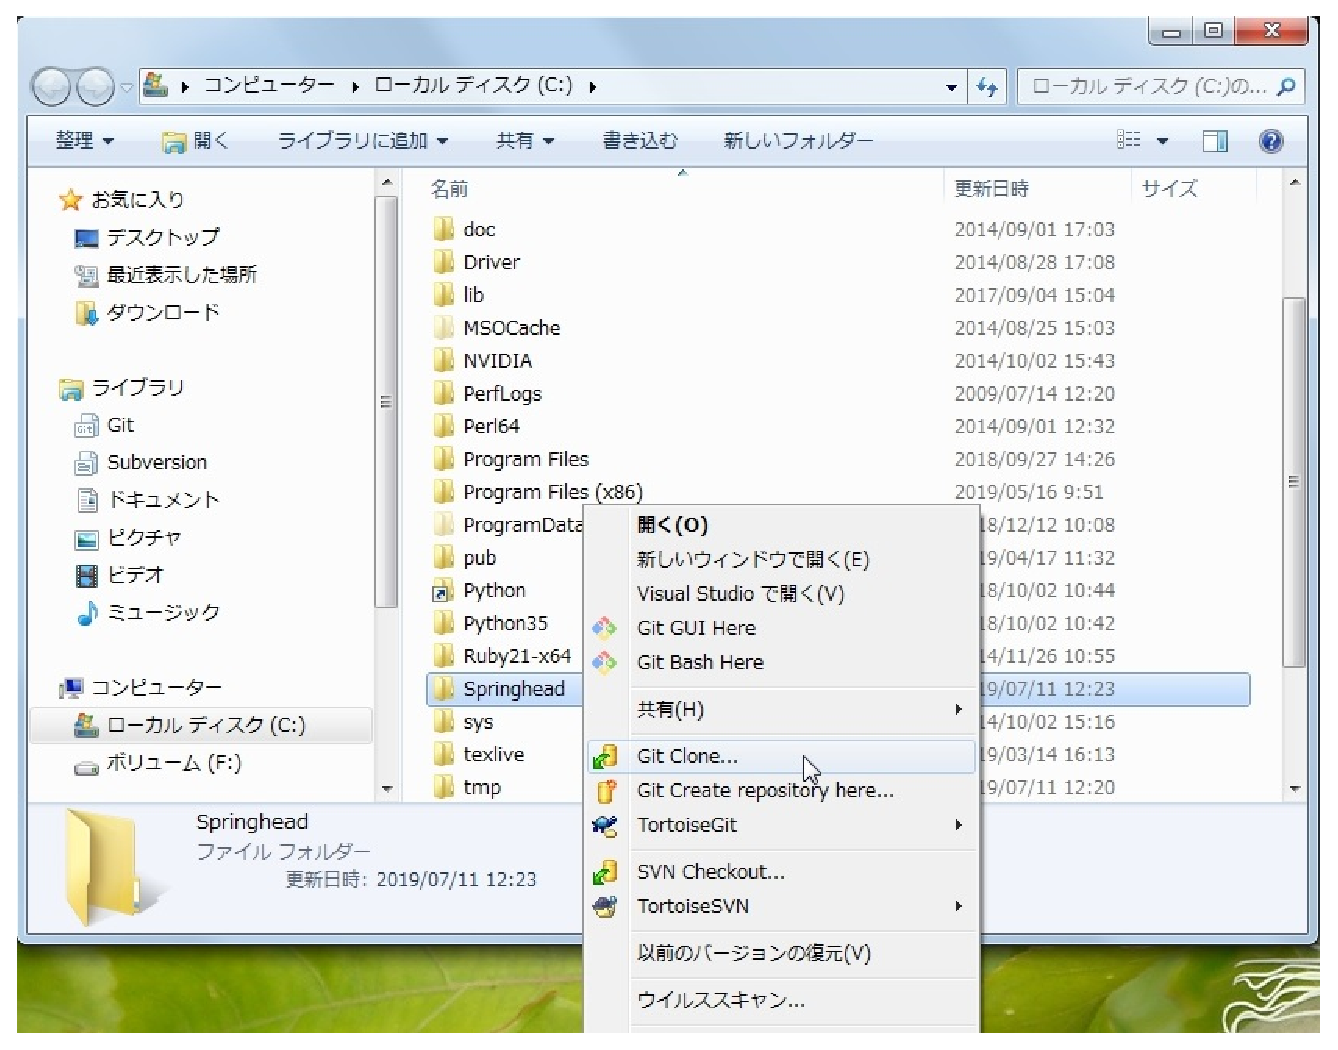
\includegraphics[width=0.5\textwidth]{fig/SpringheadClone1.eps}
	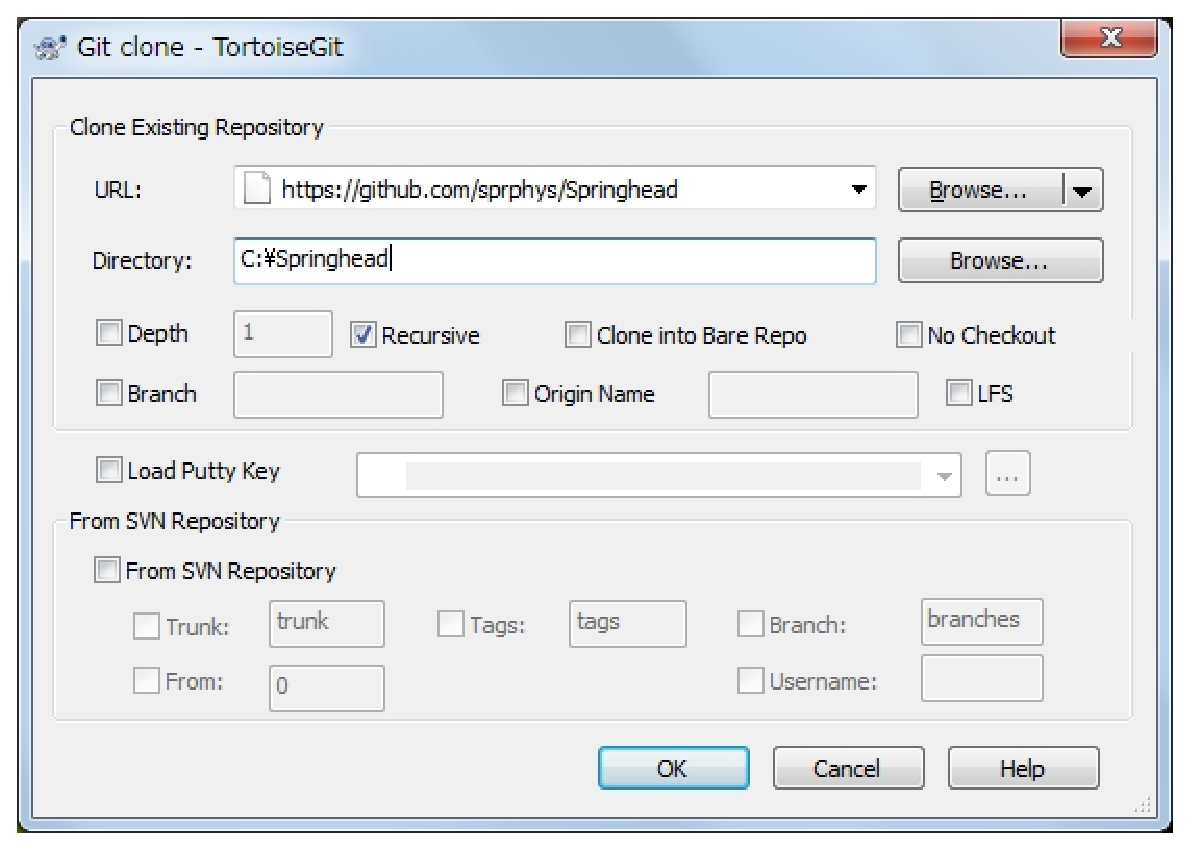
\includegraphics[width=0.4\textwidth]{fig/SpringheadClone2.eps}
	\end{center}
	\caption{Springhead\KLUDGE ダウンロード}
	\label{fig:SpringheadClone}
	\end{figure}
\end{narrow}

% end: 2.1.Download.tex
